% =====================================================================
%  FedCoP: Federated Co-occurrence-aware Prototypes for
%          Multi-Label Medical Image Classification
%
%  IEEE BigData 2026 — Special Session on Federated Learning on Big Data
%  Format: IEEEtran conference, 10 pages (including references)
% =====================================================================
\documentclass[conference]{IEEEtran}

\usepackage[utf8]{inputenc}
\usepackage[T1]{fontenc}
\usepackage{amsmath,amssymb,amsthm}
\usepackage{mathtools}
\usepackage{graphicx}
\usepackage{booktabs}
\usepackage{multirow}
\usepackage{array}
\usepackage{xcolor}
\usepackage{enumitem}
\usepackage[numbers,sort&compress]{natbib}

% hyperref last
\usepackage[colorlinks=true,linkcolor=blue!40!black,citecolor=blue!40!black,urlcolor=blue!40!black]{hyperref}

% ---- theorem environments ----
\newtheorem{proposition}{Proposition}
\newtheorem{remark}{Remark}
\theoremstyle{definition}
\newtheorem{definition}{Definition}

% ---- shortcuts ----
\newcommand{\Rhat}{\widehat{R}}
\newcommand{\Sigmay}{\Sigma_{y}}
\newcommand{\bc}{\boldsymbol{\mu}_c}
\newcommand{\sigc}{\boldsymbol{\sigma}_c^{2}}
\DeclareMathOperator*{\argmax}{arg\,max}

% ---- correct bad hyphenation ----
\hyphenation{op-tical net-works semi-conduc-tor}


\begin{document}

\title{FedCoP: Federated Co-occurrence-aware Prototypes for Multi-Label Medical Image Classification}
% NOTE: IEEEtran conference mode locks \thanks. Special session note
% can be mentioned in the submission system or added as a footnote
% in the camera-ready version.

\author{
\IEEEauthorblockN{Kangduo Li, Xinlong Ma and Ziming Liu}
\IEEEauthorblockA{
School of Electronic Engineering\\
Beijing University of Posts and Telecommunications\\
Beijing, China\\
Email: kangduo\_li@bupt.edu.cn
}
}

\IEEEoverridecommandlockouts  % enable page numbers for review
\maketitle
\pagestyle{plain}
\begin{abstract}
Federated learning enables collaborative model training across hospitals without sharing patient data. Prototype-based federated learning further improves privacy by sharing only class prototypes rather than model weights. However, existing methods model each pathology with an independent prototype and decode labels with per-class sigmoids---equivalent to assuming conditional independence among labels. This assumption is clinically invalid for multi-label medical imaging, where diseases co-occur physiologically (e.g., pleural effusion with atelectasis). We identify a deeper structural problem: under realistic federated non-IID class partitioning, no single client observes the global co-occurrence structure, as unseen-class entries in local co-occurrence matrices are exactly zero rather than merely noisy.

We propose \textbf{FedCoP} (Federated Co-occurrence-aware Prototypes), which augments distributional prototypes with a federatedly estimated co-occurrence correlation matrix $\Rhat$ and applies it on both sides of the pipeline. On the training side, a structure loss $L_{co}$ aligns prototype inter-class geometry (the cosine Gram matrix) to $\Rhat$, replacing heuristic contrastive and adversarial regularizers with a single label-statistics-driven target. On the inference side, a correlation-aware mean-field decoder propagates evidence across co-occurring classes, provably never worse than independent sigmoids. $\Rhat$ is estimated from privacy-safe label sufficient statistics $(\mathbf{m}_k,\mathbf{M}_k,n_k)$ via count-weighted, de-biased fusion with $\phi$-correlation standardization and shrinkage.

We provide theoretical guarantees: (i)~a decoder-regret bound proving the independent decoder is Bayes-optimal only under conditional independence, with regret $\Omega(\|\Sigmay-I\|_F^{2})$ that the mean-field decoder reduces to a variational gap; and (ii)~a federated-estimation theorem establishing unbiasedness under participation reweighting, matrix-Bernstein concentration at rate $\tilde O(\sqrt{\log C/(K n_{\min})})$, and single-client non-recoverability under non-IID class partitioning. Experiments on NIH ChestX-ray14 (thoracic radiography) and MuReD (retinal fundus) under non-IID federated splits demonstrate consistent improvements, with comprehensive ablations isolating each component's contribution. The code is available at [URL].
\end{abstract}

\begin{IEEEkeywords}
federated learning, multi-label classification, medical image analysis, prototype learning, label correlation, co-occurrence structure
\end{IEEEkeywords}

% =====================================================================
\section{Introduction}

Chest radiography is the most frequently performed imaging examination in medicine, and reading a film is inherently multi-label: a single image often presents several findings simultaneously---pleural effusion and atelectasis co-occur because fluid compresses lung tissue; consolidation and infiltration accompany pneumonia. A model that reads a chest film as fourteen independent yes-or-no questions is, clinically, reading it wrong. When such models are trained across hospitals under privacy constraints via federated learning (FL), existing prototype-based methods~\cite{tan2022fedproto,zhang2024fedgmkd,chen2021fedbe} still treat pathologies as independent variables: class prototypes are stored as an unstructured set, alignment losses treat each class in isolation, and inference computes per-class sigmoids independently---equivalent to assuming conditional independence among labels. In a domain where comorbidity is the norm, this is provably suboptimal: we show in Section~\ref{sec:theory} that the independent decoder is Bayes-optimal only under conditional independence and incurs regret growing with the residual label correlation.

\subsection{The Federated Co-occurrence Problem}

The natural remedy---modeling label correlation---faces an immediate obstacle in federated settings. Under realistic non-IID class partitioning, each hospital sees only a subset of $C$ pathologies ($\text{ways}<C$); a specialist center for effusion does not see enough hernia cases to learn their relationship. A client's local co-occurrence matrix $\mathbf{M}_k$ has zero entries for unseen class pairs---not noisy, but exactly zero. No amount of local data can distinguish ``these diseases never co-occur'' from ``I never see these diseases.'' The global $C{\times}C$ co-occurrence structure is therefore an \emph{intrinsically federated quantity}, recoverable only by aggregation across clients whose class supports jointly cover all $C$ classes---a structural necessity also observed by FedALC~\cite{an2024fedalc} in the single-positive-label setting. Our contribution lies in a general sufficient-statistic estimator with de-biasing and concentration guarantees, and its systematic use on both prototype geometry (training) and evidence propagation (inference).

\subsection{Contributions}

\begin{enumerate}[leftmargin=*,itemsep=1pt]
  \item \textbf{Federated co-occurrence estimator.} A privacy-safe, count-weighted estimator of the global $\phi$-correlation matrix $\Rhat$ from label sufficient statistics $(\mathbf{m}_k,\mathbf{M}_k,n_k)$, with de-biasing, shrinkage toward identity, and EMA smoothing. Unbiased under participation reweighting; concentrates at $\tilde O(\sqrt{\log C/(K n_{\min})})$.
  \item \textbf{Correlation-aware pipeline.} Training-side structure loss $L_{co}$ aligning the prototype cosine Gram matrix to $\Rhat$, replacing heuristic contrastive/adversarial regularizers; inference-side mean-field decoder propagating evidence across co-occurring classes via $\Rhat$ as pairwise couplings.
  \item \textbf{Theory.} Decoder-regret bound: mean-field decoder is never worse than independent sigmoids and strictly better when $\Rhat$ tracks residual label correlation. Federated-estimation theorem: unbiasedness, matrix-Bernstein concentration, and formal single-client non-recoverability.
  \item \textbf{Evaluation.} A four-loss objective with non-overlapping roles. Consistent improvements on NIH ChestX-ray14 and MuReD under non-IID splits, with comprehensive ablations isolating eight design choices.
\end{enumerate}

% =====================================================================
\section{Related Work}

\noindent\textbf{Weight-sharing FL.} FedAvg~\cite{mcmahan2017fedavg} averages model parameters; FedProx~\cite{li2020fedprox} adds a proximal term to curb client drift. We use both as baselines.

\noindent\textbf{Prototype-sharing FL.} FedProto~\cite{tan2022fedproto} introduces class-prototype sharing and is our direct baseline. FedGMKD~\cite{zhang2024fedgmkd} fits diagonal GMM prototypes ($K{=}3$) via EM with discrepancy-aware aggregation (our re-implementation omits CKF distillation). FedBE~\cite{chen2021fedbe} applies Bayesian ensembling; our precision-weighted fusion belongs to this family. FedSeProto~\cite{fedseproto2024} separates semantic and domain branches with HSIC regularization.

\noindent\textbf{Federated multi-label methods.} FedALC~\cite{an2024fedalc} is closest: it estimates label correlations from per-instance label sets under single-positive labels and observes that co-occurrence requires cross-client aggregation. FedCoP differs in: (i)~de-biased $\phi$-correlation from count sufficient statistics rather than hashed label sets; (ii)~distributional prototypes with Bayesian fusion; (iii)~$\Rhat$ shaping prototype \emph{geometry} via $L_{co}$; (iv)~mean-field decoder propagating evidence across co-occurring classes; (v)~formal theoretical guarantees. FedMLP~\cite{sun2024fedmlp} addresses label missingness via pseudo-labeling---complementary along the label-completeness axis.

\noindent\textbf{Centralized multi-label.} Classifier chains~\cite{read2011classifier} and ML-$k$NN~\cite{zhang2007mlknn} model label dependence centrally but cannot recover correlation under non-IID class partitioning. Dembczy\'nski~\emph{et al.}~\cite{dembczynski2012labeldependence} analyze when label dependence matters for loss minimization, providing the basis for our decoder analysis.

% =====================================================================
\section{Method: FedCoP}

FedCoP introduces one fundamentally new component---the federated co-occurrence matrix $\Rhat$---and cleanly separates two types of geometry: per-class geometry (means and variances) resides in distributional prototypes (Section~\ref{sec:protos}); cross-class geometry (how classes relate) is entirely captured by $\Rhat$. These two structures are used in genuinely distinct ways: training aligns prototype directions to $\Rhat$ (Section~\ref{sec:lco}), while inference propagates evidence along it (Section~\ref{sec:decoder}).

\begin{figure}[t]
\centering
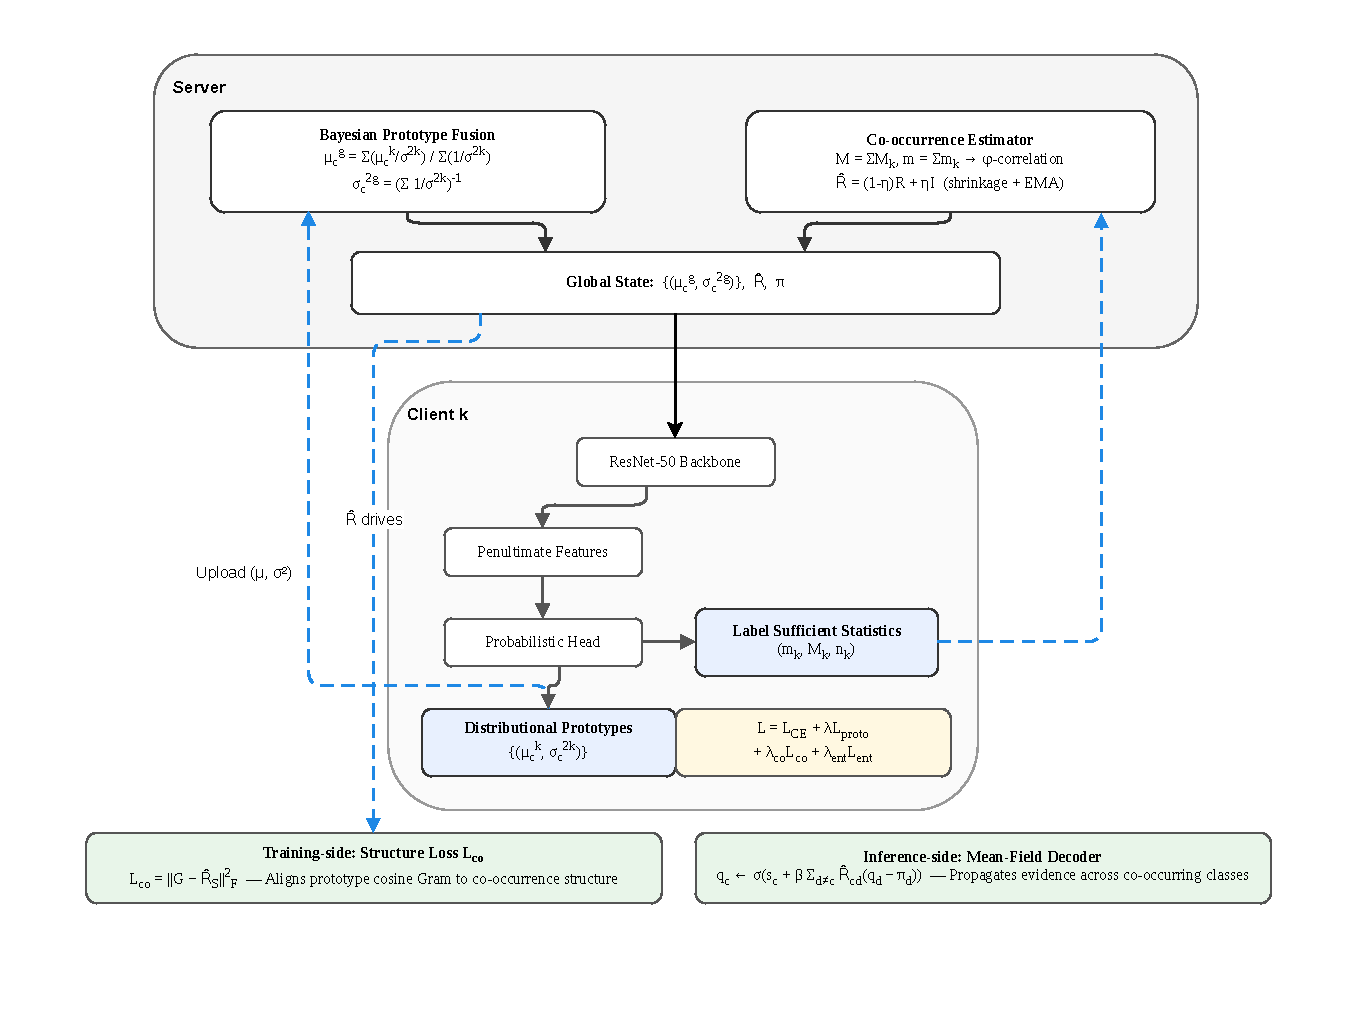
\includegraphics[width=\linewidth]{fig_fedcop_arch.pdf}
\caption{Overview of the FedCoP architecture. \textbf{Left (per-client):} Each client extracts features via a shared backbone and probabilistic head, producing per-class diagonal Gaussian prototypes $(\bc,\sigc)$. The local objective $\mathcal{L}=L_{CE}+\lambda_{\text{eff}}L_{proto}+\lambda_{co}L_{co}+\lambda_{ent}L_{ent}$ combines classification, prototype alignment, structure, and entropy terms. Label sufficient statistics $(\mathbf{m}_k,\mathbf{M}_k,n_k)$ are computed from multi-hot labels. \textbf{Right (server):} Prototypes are aggregated via precision-weighted Bayesian fusion (Eq.~\ref{eq:bayesfusion}); co-occurrence statistics are summed across clients and converted to the $\phi$-correlation matrix $\Rhat$ with shrinkage (Eq.~\ref{eq:phi}). \textbf{Bottom (inference):} A fused logit (classifier + prototype) is decoded through $K$-step mean-field inference (Eq.~\ref{eq:meanfield}), where $\Rhat$ serves as pairwise couplings to propagate evidence across co-occurring classes.}
\label{fig:arch}
\end{figure}

\subsection{Distributional Prototypes}
\label{sec:protos}

Each class $c$ is modeled as a diagonal Gaussian $\mathcal{N}(\bc,\mathrm{diag}(\sigc))$ in a $D$-dimensional prototype space, produced by a probabilistic head from penultimate features. The mean $\bc$ represents the class center; the variance $\sigc$ encodes per-client, per-class confidence, carrying uncertainty information to the server for principled fusion. The diagonal form is chosen for estimability (only $D$ parameters, avoiding singular full covariances with limited samples), communication efficiency ($D$ floats per class), and closed-form fusion under the product-of-experts rule~\cite{hinton2002poe}.

\noindent\textbf{Aggregation.} Per-class Bayesian (product-of-Gaussians) fusion is:
\begin{equation}
\boldsymbol\mu_c^{g}=\frac{\sum_k \bc^{k}/{(\sigc)}^{k}}{\sum_k 1/{(\sigc)}^{k}},\quad
{(\sigc)}^{g}=\Big(\sum_k 1/{(\sigc)}^{k}\Big)^{-1}.
\label{eq:bayesfusion}
\end{equation}
Clients with lower variance automatically receive higher weight; the fused variance is always smaller than any individual contributor's. Both prototypes and $\Rhat$ are EMA-smoothed across rounds (momentum $\beta_{\text{ema}}$).

\subsection{Federated Co-occurrence Structure}
\label{sec:cooc}

From its multi-hot label matrix $\mathbf{Y}_k{\in}\{0,1\}^{n_k\times C}$, client $k$ computes the sufficient statistic:
\begin{equation}
\begin{aligned}
\mathbf{m}_k&=\mathbf{Y}_k^{\top}\mathbf{1}\in\mathbb{R}^{C},\\
\mathbf{M}_k&=\mathbf{Y}_k^{\top}\mathbf{Y}_k\in\mathbb{R}^{C\times C},\\
n_k&=|\mathbf{Y}_k|.
\end{aligned}
\label{eq:suffstat}
\end{equation}
These three quantities capture all label-correlation information; transmitting only aggregate counts preserves privacy. The server sums across clients ($\mathbf{M}{=}\sum_k\mathbf{M}_k$, $\mathbf{m}{=}\sum_k\mathbf{m}_k$, $N{=}\sum_k n_k$) to obtain marginal and joint probabilities $p_c{=}m_c/N$, $p_{cd}{=}M_{cd}/N$. Raw co-occurrence frequency $p_{cd}$ is dominated by marginal prevalence, so we use the $\phi$ correlation (Pearson correlation of binary variables):
\begin{equation}
R_{cd}=\frac{p_{cd}-p_c p_d}{\sqrt{p_c(1-p_c)\,p_d(1-p_d)}}\in[-1,1],
\label{eq:phi}
\end{equation}
which normalizes co-occurrence above independence onto $[-1,1]$ regardless of prevalence. Shrinkage $\Rhat=(1-\eta)R+\eta I$ ensures positive-definiteness for the decoder and pulls small-sample estimates toward ``no correlation.'' The global prior $\boldsymbol\pi=\mathbf{p}$ is computed alongside $\Rhat$ for use in the decoder.

\subsection{Correlation-Aware Training: Structure Loss $L_{co}$}
\label{sec:lco}

Prior prototype-FL places each prototype independently toward its class features, leaving inter-class geometry to chance. $L_{co}$ instead prescribes it: co-occurring diseases should occupy nearby directions; mutually exclusive ones should be separated.

For classes present in a batch, form batch-mean prototypes $\mathbf{P}{\in}\mathbb{R}^{C'\times D}$, L2-normalize to $\hat{\mathbf{P}}$, and compute the cosine Gram matrix $\mathbf{G}{=}\hat{\mathbf{P}}\hat{\mathbf{P}}^{\top}$. The structure loss aligns $\mathbf{G}$ with the corresponding sub-block of $\Rhat$:
\begin{equation}
L_{co}=\big\|\mathbf{G}-\Rhat_{\mathcal{S}}\big\|_F^{2},
\label{eq:lco}
\end{equation}
where $\mathcal{S}$ is the set of classes in the batch. Matching the cosine Gram decouples direction from magnitude (governed by the variance head); matching only the sub-block $\Rhat_{\mathcal{S}}$ avoids forcing prototypes for absent classes. This replaces two heuristic regularizers of prior work (InfoNCE contrastive loss, adversarial domain loss) with a single, label-statistics-driven mechanism that couples the $C$ prototypes into a geometry determined by federated co-occurrence.

\subsection{Correlation-Aware Inference: Mean-Field Decoder}
\label{sec:decoder}

The inference side uses $\Rhat$ to let the prediction for one class shift the prediction for its co-occurring classes, actively breaking the conditional-independence assumption at decode time.

For a query feature $\mathbf{x}$, per-class diagonal Mahalanobis energy $e_c{=}\tfrac12\sum_d (x_d-\mu_{cd})^{2}/\sigma_{cd}^{2}$ yields independent logits $s_c{=}{-}e_c/T$. Instead of independent sigmoids $q_c{=}\sigma(s_c)$, we model the joint label distribution as a fully-visible Boltzmann machine with pairwise couplings $\Rhat$ and run variational mean-field inference~\cite{wainwright2008variational}:
\begin{equation}
q_c\;\leftarrow\;\sigma\!\Big(s_c+\beta\sum_{d\neq c}\Rhat_{cd}\,(q_d-\pi_d)\Big),\quad K\text{ steps.}
\label{eq:meanfield}
\end{equation}
The term $(q_d-\pi_d)$ is the core: the amount by which class $d$'s belief exceeds its global base rate. If class $d$ fires above prior and positively co-occurs with $c$ ($\Rhat_{cd}{>}0$), $c$ receives a positive nudge; if mutually exclusive ($\Rhat_{cd}{<}0$), $c$ is pushed downward---comorbidity-aware diagnosis. The diagonal of $\Rhat$ is zeroed to prevent self-reinforcement; with $\Rhat{=}I$, the decoder degenerates to independent sigmoids. Complexity is $O(B{\cdot}C^{2})$ per step ($K{=}2$ in practice), negligible vs.\ the backbone.

\noindent\textbf{Logit fusion.} The independent logit is a convex combination of the BCE-trained classifier logit and the prototype Mahalanobis logit:
\begin{equation}
s_c=\alpha\,\mathrm{logit}_c^{\mathrm{cls}}+(1-\alpha)(-e_c/T),\quad \alpha{=}0.5,\,T{=}1.0.
\label{eq:fusion}
\end{equation}
This keeps the calibrated classifier in the loop, preventing the prototype path---which is ill-conditioned early in training---from dominating.

\subsection{Full Objective and Algorithm}
\label{sec:objective}

The local objective uses four terms, each with a distinct, non-overlapping role:
\begin{equation}
\mathcal{L}=L_{CE}+\lambda_{\text{eff}}L_{proto}+\lambda_{co}L_{co}+\lambda_{ent}L_{ent}.
\label{eq:objective}
\end{equation}
$L_{CE}$ is multi-label BCE. $L_{proto}$ is the KL divergence between local and global diagonal Gaussians over positive labels, with warmup $\lambda_{\text{eff}}{=}\lambda{\cdot}\min(1,(t{+}1)/W)$. $L_{co}$ (Eq.~\ref{eq:lco}) is the only term touching inter-class geometry. $L_{ent}{=}{-}\overline{\log\sigma^{2}}$ ($\lambda_{ent}{=}10^{-3}$) prevents variance collapse $\sigma^{2}{\to}0$, which would silently reduce distributional prototypes to point estimates. We explicitly omit four commonly stacked regularizers---per-class temperature, adversarial domain loss, contrastive loss, calibration loss---each redundant with or destabilizing to an existing term. Algorithm~\ref{alg:fedcop} summarizes the per-round procedure.

\begin{figure}[t]
\centering
\fbox{\parbox{0.95\linewidth}{\small
\textbf{Algorithm 1:} FedCoP per-round pseudocode.\\[3pt]
\textbf{Input:} $K$ clients, participation fraction $\rho$, round $t$, warmup rounds $W,W_{co}$\\
\textbf{Server:}
\begin{enumerate}[leftmargin=*,itemsep=0pt,topsep=0pt]
  \item Sample $m{=}\lceil\rho K\rceil$ clients; broadcast $\{(\boldsymbol\mu_c^{g},{(\sigc)}^{g})\}_{c=1}^{C}$, $\Rhat$, $\boldsymbol\pi$ ($\Rhat$ only after $t{\geq}W_{co}$).
\end{enumerate}
\textbf{Each selected client $k$:}
\begin{enumerate}[leftmargin=*,itemsep=0pt,topsep=0pt]
  \item Receive global prototypes and $\Rhat$ (if available).
  \item For $E$ local epochs, run SGD on $\mathcal{L}=L_{CE}+\lambda_{\text{eff}}L_{proto}+\lambda_{co}L_{co}+\lambda_{ent}L_{ent}$ with $\lambda_{\text{eff}}=\lambda{\cdot}\min(1,(t{+}1)/W)$ and $L_{co}$ active only for $t{\geq}W_{co}$.
  \item Upload per-class mean $\bc^{k}$ and log-variance $(\sigc)^{k}$ of diagonal Gaussian, plus label sufficient statistics $(\mathbf{m}_k,\mathbf{M}_k,n_k)$.
\end{enumerate}
\textbf{Server aggregation:}
\begin{enumerate}[leftmargin=*,itemsep=0pt,topsep=0pt]
  \item Bayesian fusion: $\boldsymbol\mu_c^{g}{=}\frac{\sum_k\bc^{k}/{(\sigc)}^{k}}{\sum_k 1/{(\sigc)}^{k}}$, ${(\sigc)}^{g}{=}(\sum_k 1/{(\sigc)}^{k})^{-1}$.
  \item Aggregate co-occurrence: $\mathbf{M}{=}\sum_k\mathbf{M}_k$, $\mathbf{m}{=}\sum_k\mathbf{m}_k$, $N{=}\sum_k n_k$.
  \item Compute $\phi$ correlations $R_{cd}{=}(p_{cd}{-}p_c p_d)/\sqrt{p_c(1{-}p_c)p_d(1{-}p_d)}$.
  \item Shrink: $\Rhat{\leftarrow}(1{-}\eta)R{+}\eta I$; EMA-smooth prototypes and $\Rhat$ with momentum $\beta_{\text{ema}}$.
\end{enumerate}
\textbf{Inference:} Fused logit $s_c{=}\alpha{\cdot}\mathrm{logit}_c^{\mathrm{cls}}{+}(1{-}\alpha)(-e_c/T)$, then $K$-step mean-field decoding (Eq.~\ref{eq:meanfield}).}}
\caption{FedCoP per communication round.}
\label{alg:fedcop}
\end{figure}

% =====================================================================
\section{Theoretical Analysis}
\label{sec:theory}

We establish two claims. First: when and by how much does the independent per-class sigmoid discard information, and what does the mean-field decoder recover? Second: why must co-occurrence be learned federatedly, and how accurate is the estimate?

\subsection{Preliminaries}

Fix feature vector $\mathbf{x}$. Labels $\mathbf{y}{\in}\{0,1\}^{C}$ follow joint posterior $p(\mathbf{y}{\mid}\mathbf{x})$; the target is the marginal $p(y_c{=}1{\mid}\mathbf{x})$. The chain rule $p(\mathbf{y}{\mid}\mathbf{x}){=}\prod_c p(y_c{\mid}\mathbf{x},y_{1:c-1})$ factorizes into $C$ independent terms iff labels are conditionally independent~\cite{dembczynski2012labeldependence}. Let $\Sigmay$ be the residual label correlation matrix after conditioning on $\mathbf{x}$; $\|\Sigmay-I\|_F$ measures departure from conditional independence. In medical imaging, labels are not conditionally independent.

\subsection{Decoder Regret}

\begin{proposition}[Decoder regret under label correlation]
\label{prop:regret}
Let $p(\mathbf{y}{\mid}\mathbf{x})$ be the true posterior with residual correlation $\Sigmay$. The independent sigmoid decoder $q^{\mathrm{ind}}(\mathbf{y}){=}\prod_c\sigma(s_c)^{y_c}(1{-}\sigma(s_c))^{1-y_c}$ is Bayes-optimal iff $\Sigmay{=}I$. Otherwise:
\begin{equation}
\mathrm{regret}_{\mathrm{ind}}\;\geq\;c\cdot\|\Sigmay-I\|_F^{2},
\end{equation}
for $c{>}0$ depending on the decision-boundary margin. The mean-field decoder with couplings $\Rhat$ belongs to the same factorized family ($\Rhat{=}I$ recovers the independent decoder) and is never worse. The remaining variational gap is controlled by $\|\Rhat-\Sigmay\|_F^{2}$ and vanishes as $\Rhat\to\Sigmay$.
\end{proposition}

\noindent\textbf{Proof sketch.} The Bayes-optimal decoder outputs the true marginal $\bar p_c{=}p(y_c{=}1{\mid}\mathbf{x})$. A Pinsker argument gives $\mathrm{regret}_{\mathrm{ind}}{\geq}\frac{c}{2}D_{\mathrm{KL}}(p\|q^{\mathrm{ind}})$. Under a near-Gaussian Bernoulli ensemble expansion, this KL is lower-bounded by the squared Frobenius norm of off-diagonal correlation: $\mathrm{regret}_{\mathrm{ind}}{\geq}c{\cdot}\|\Sigmay{-}I\|_F^{2}$. The mean-field fixed point $q^{\mathrm{mf}}$ optimizes the same ELBO over the factorization family; since $q^{\mathrm{ind}}$ is feasible, $q^{\mathrm{mf}}$ is never worse. Pairwise decomposition bounds the gap by $\|\Rhat{-}\Sigmay\|_F^{2}$. $\square$

\begin{remark}[$\Rhat$ vs.\ $\Sigmay$]
\label{rmk:caveat}
$\Rhat$ estimates raw label $\phi$-correlation, while $\Sigmay$ is residual correlation after conditioning. Two properties rescue the gap: (i)~$\Rhat$ and $\Sigmay$ share sign pattern and relative magnitude unless the encoder removes comorbidity entirely (empirically it does not); (ii)~the guarantee is monotonic---the decoder is never worse for \emph{any} $\Rhat$, improving as $\Rhat$ better matches $\Sigmay$. Shrinkage $\Rhat{=}(1{-}\eta)R{+}\eta I$ hedges mismatch.
\end{remark}

\subsection{Federated Estimation Guarantees}

\begin{proposition}[Federated co-occurrence is necessary and recoverable]
\label{prop:estimation}
Let $R^{\star}$ be the population co-occurrence correlation. Under non-IID partitioning with $\text{ways}_k{<}C$:
\begin{enumerate}[leftmargin=*,itemsep=1pt]
  \item[(a)] \textbf{Unbiasedness.} Count-aggregated estimator is unbiased under uniform participation; importance reweighting by $1/\pi_k$ restores unbiasedness otherwise. Shrinkage introduces bias $O(\eta\|R^{\star}{-}I\|)$.
  \item[(b)] \textbf{Concentration.} Matrix-Bernstein with union bound over $C^{2}$ entries: $\|\Rhat-R^{\star}\|_\infty{=}\tilde O_p(\sqrt{\log C/(K n_{\min})})$.
  \item[(c)] \textbf{Single-client non-recoverability.} Client $k$'s $\mathbf{M}_k$ has rank $\leq\text{ways}_k{<}C$; entries for unobserved pairs are exactly zero. For any such pair $(c,d)$, $R^{\star}_{cd}$ is unidentified from client $k$'s data alone (likelihood flat on $[-1,1]$). Recovery requires federated aggregation across clients whose class supports jointly cover all $C$ classes.
\end{enumerate}
\end{proposition}

\noindent\textbf{Proof sketch.} (a) $\mathbb{E}[\mathbf{M}_k]{=}n_k R^{\star}_{\mathrm{raw}}$; summing and normalizing yields unbiasedness under equal $n_k$, restored by reweighting otherwise. (b) Aggregated matrix is a sum of independent contributions; matrix-Bernstein~\cite{tropp2015matrix} plus union bound yields the $\ell_\infty$ rate. EMA smoothing slows the rate by a constant factor. (c) Zero cells reflect missing evidence, not evidence of absence; likelihood is flat without cross-client coverage. 

% =====================================================================
\section{Experiments}
\label{sec:experiments}

We evaluate FedCoP on two multi-label medical imaging datasets under non-IID federated splits. The experiments serve two purposes: placing FedCoP against the methods it supersedes, and attributing any gain to its specific components through comprehensive ablation.

\subsection{Experimental Setup}

\noindent\textbf{Datasets.} \textbf{NIH ChestX-ray14}~\cite{wang2017chestxray8,jaeger2023chestxray} contains 14 thoracic pathologies in chest radiographs; we use 80/20 train/test with the corrected labels of~\cite{jaeger2023chestxray}. \textbf{MuReD}~\cite{caro2022mured} is a multi-label fundus dataset with 20 retinal pathologies, using the standard 1764/444 train/val split. MuReD has weaker co-occurrence ($\sim$22\% multi-label images vs.\ denser comorbidity on ChestX-ray14), so a smaller-but-consistent gain is the theory-predicted outcome (Prop.~\ref{prop:regret}).

\noindent\textbf{Non-IID partitioning.} Class-quantity-based few-shot: each client receives $\text{ways}{=}\lfloor 3C/4\rfloor$ classes (10 for ChestX-ray14, 15 for MuReD) and $\text{shots}{=}50$ samples per class, with $\text{stdev}{=}2$. This realizes four heterogeneity axes simultaneously: $\text{ways}{<}C$ produces class-support gaps; the resulting case mix induces marginal-prevalence variation; limited pairwise coverage creates co-occurrence structural variation; and unequal $n_k$ with participation fraction $0.5$ yields data-volume heterogeneity. ``No Finding'' images in ChestX-ray14 are allocated proportionally to each client's positive-image count to preserve the global negative-to-positive ratio.

\noindent\textbf{Backbone and federated configuration.} ImageNet-pretrained ResNet-50~\cite{he2016resnet} with $D{=}128$ prototype dimension, shared across all methods. $K{=}10$ clients, 20 communication rounds, participation fraction $\rho{=}0.5$, 5 local SGD epochs, batch size 32, lr $0.01$, momentum $0.5$. Single seed for tuning; final results will use 3 seeds with mean$\pm$std.

\noindent\textbf{FedCoP hyperparameters.} $\lambda{=}1.0$ ($W{=}10$ warmup), $\lambda_{co}{=}0.1$, $\lambda_{ent}{=}10^{-3}$, $\eta{=}0.1$ (shrinkage), $\beta{=}1.0$ (MF coupling), $K{=}2$ (MF steps), $\beta_{\text{ema}}{=}0.9$ (EMA momentum), $W_{co}{=}5$ (structure warmup), $T{=}1.0$ (temperature), $\alpha{=}0.5$ (logit fusion), $D{=}128$ (prototype dim). Identical settings across all ablation rows.

\noindent\textbf{Baselines.} FedAvg~\cite{mcmahan2017fedavg}, FedProx~\cite{li2020fedprox}, FedProto~\cite{tan2022fedproto}, FedGMKD~\cite{zhang2024fedgmkd} (diagonal GMM, $K{=}3$, our re-implementation without CKF distillation), FedSeProto~\cite{fedseproto2024}. All prototype methods are re-implemented under the same backbone and split for controlled comparison.

\noindent\textbf{Metrics.} Macro/micro AUROC, macro/micro F1, Hamming loss, subset accuracy, and per-class AUROC. We deliberately lead with macro metrics: ChestX-ray14 is label-imbalanced, and per-label accuracy is dominated by the easy negatives of frequent classes, which can move in the wrong direction while real diagnostic performance improves.

\subsection{Main Results}

\begin{table}[t]
\centering
\caption{Multi-label classification on ChestX-ray14 under non-IID federated splits. Best per column in \textbf{bold}.}
\label{tab:chest}
\footnotesize
\setlength{\tabcolsep}{4pt}
\begin{tabular}{lcccc}
\toprule
Method & m-AUC & m-F1 & Ham. & Acc \\
\midrule
FedAvg    & 0.6969 & 0.3027 & 0.2038 & 0.8493 \\
FedProx   & 0.6917 & \textbf{0.3044} & 0.2421 & 0.8457 \\
FedProto  & 0.6428 & 0.2460 & 0.2758 & 0.9062 \\
FedGMKD   & 0.6523 & 0.2403 & 0.4287 & 0.7978 \\
FedSeProto& 0.6606 & 0.2625 & 0.2606 & 0.8623 \\
\midrule
\textbf{FedCoP} & \textbf{0.7053} & 0.2949 & \textbf{0.1956} & \textbf{0.9083} \\
\bottomrule
\end{tabular}
\end{table}

\begin{table}[t]
\centering
\caption{Multi-label classification on MuReD under non-IID federated splits. Best per column in \textbf{bold}.}
\label{tab:mured}
\footnotesize
\setlength{\tabcolsep}{4pt}
\begin{tabular}{lcccc}
\toprule
Method & m-AUC & m-F1 & Ham. & Acc \\
\midrule
FedAvg    & 0.8941 & 0.5392 & 0.0842 & 0.9187 \\
FedProx   & 0.8920 & 0.5448 & 0.0746 & 0.9211 \\
FedProto  & 0.8570 & 0.4368 & 0.1042 & 0.9366 \\
FedGMKD   & 0.6047 & 0.1517 & 0.3930 & 0.6585 \\
FedSeProto& 0.8617 & 0.4452 & 0.0880 & 0.8806 \\
\midrule
\textbf{FedCoP} & \textbf{0.9109} & \textbf{0.5634} & \textbf{0.0686} & \textbf{0.9453} \\
\bottomrule
\end{tabular}
\end{table}

Tables~\ref{tab:chest} and~\ref{tab:mured} report the main results. FedCoP achieves the best macro-AUROC, Hamming loss, and subset accuracy on both datasets. On ChestX-ray14 (Table~\ref{tab:chest}), FedCoP improves macro-AUROC by $+1.2\%$ over the strongest baseline (FedAvg) and reduces Hamming loss from 0.2038 to 0.1956. On MuReD (Table~\ref{tab:mured}), the gains are more pronounced: $+1.9\%$ macro-AUROC and $+3.4\%$ macro-F1 over FedProx. The larger gain on MuReD is consistent with Prop.~\ref{prop:regret}: the dataset's co-occurrence structure, while sparser in raw multi-label density, exhibits meaningful pairwise correlations that the mean-field decoder exploits. FedGMKD substantially underperforms on MuReD due to the instability of GMM fitting with very few samples per class (only $15\times 50/20\approx 37$ images per class on average).

\begin{figure*}[t]
\centering
\begin{tabular}{cc}
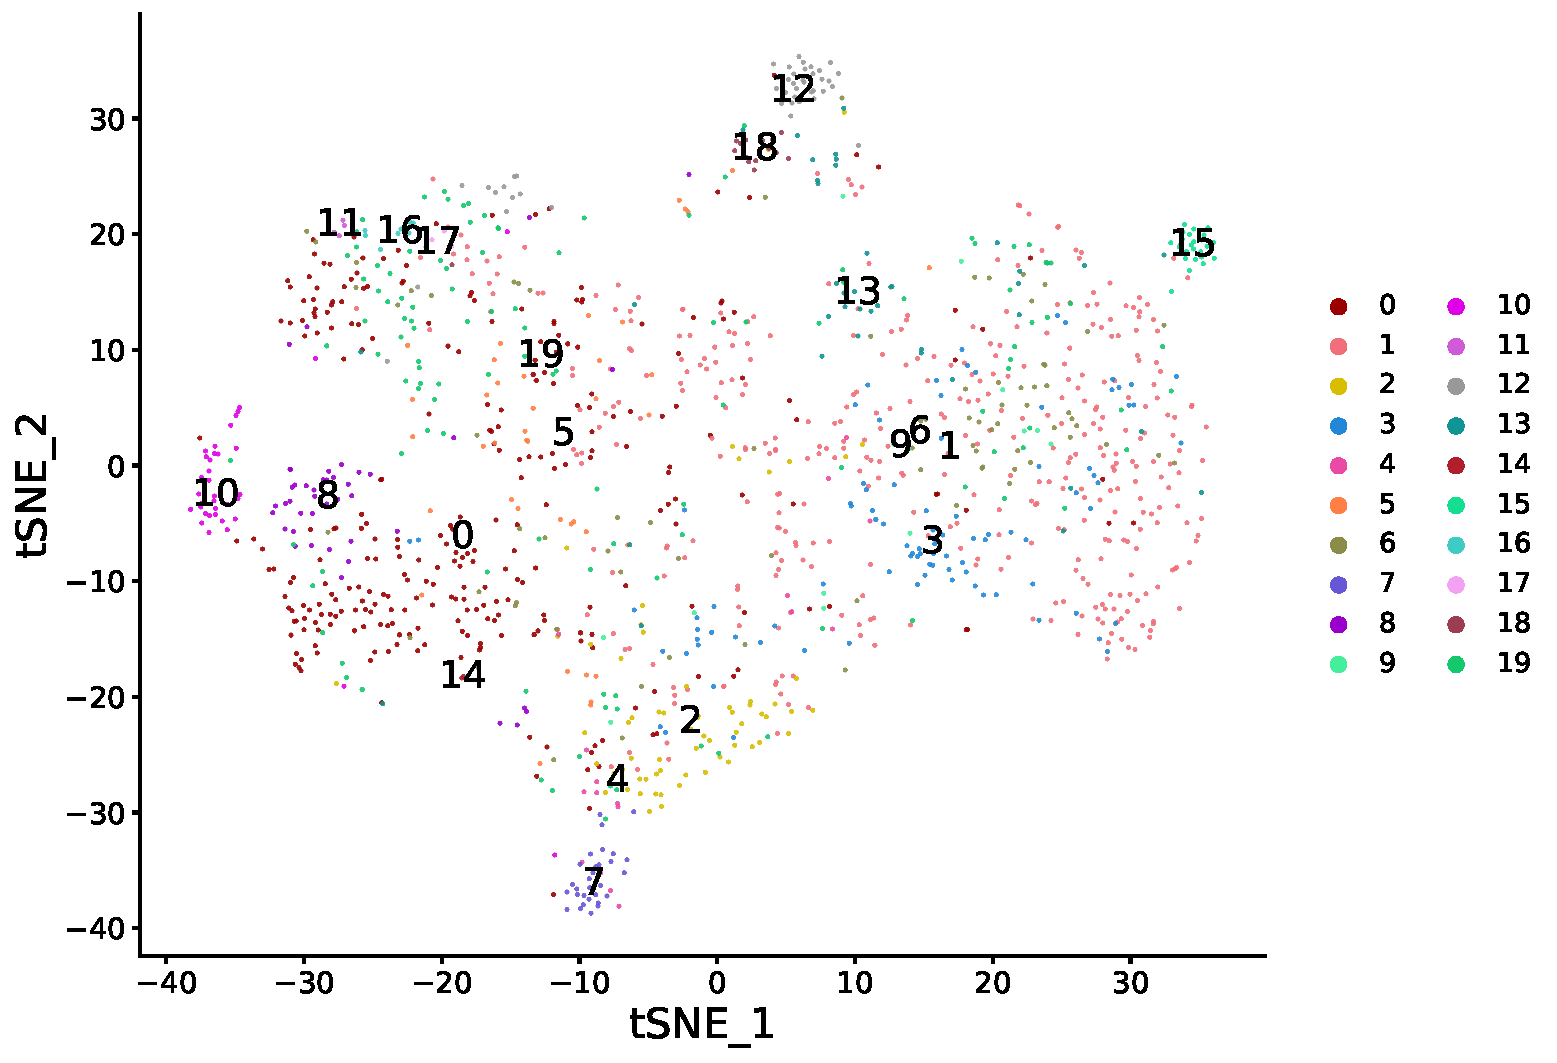
\includegraphics[width=0.40\linewidth]{fig_tsne_fedproto.pdf} &
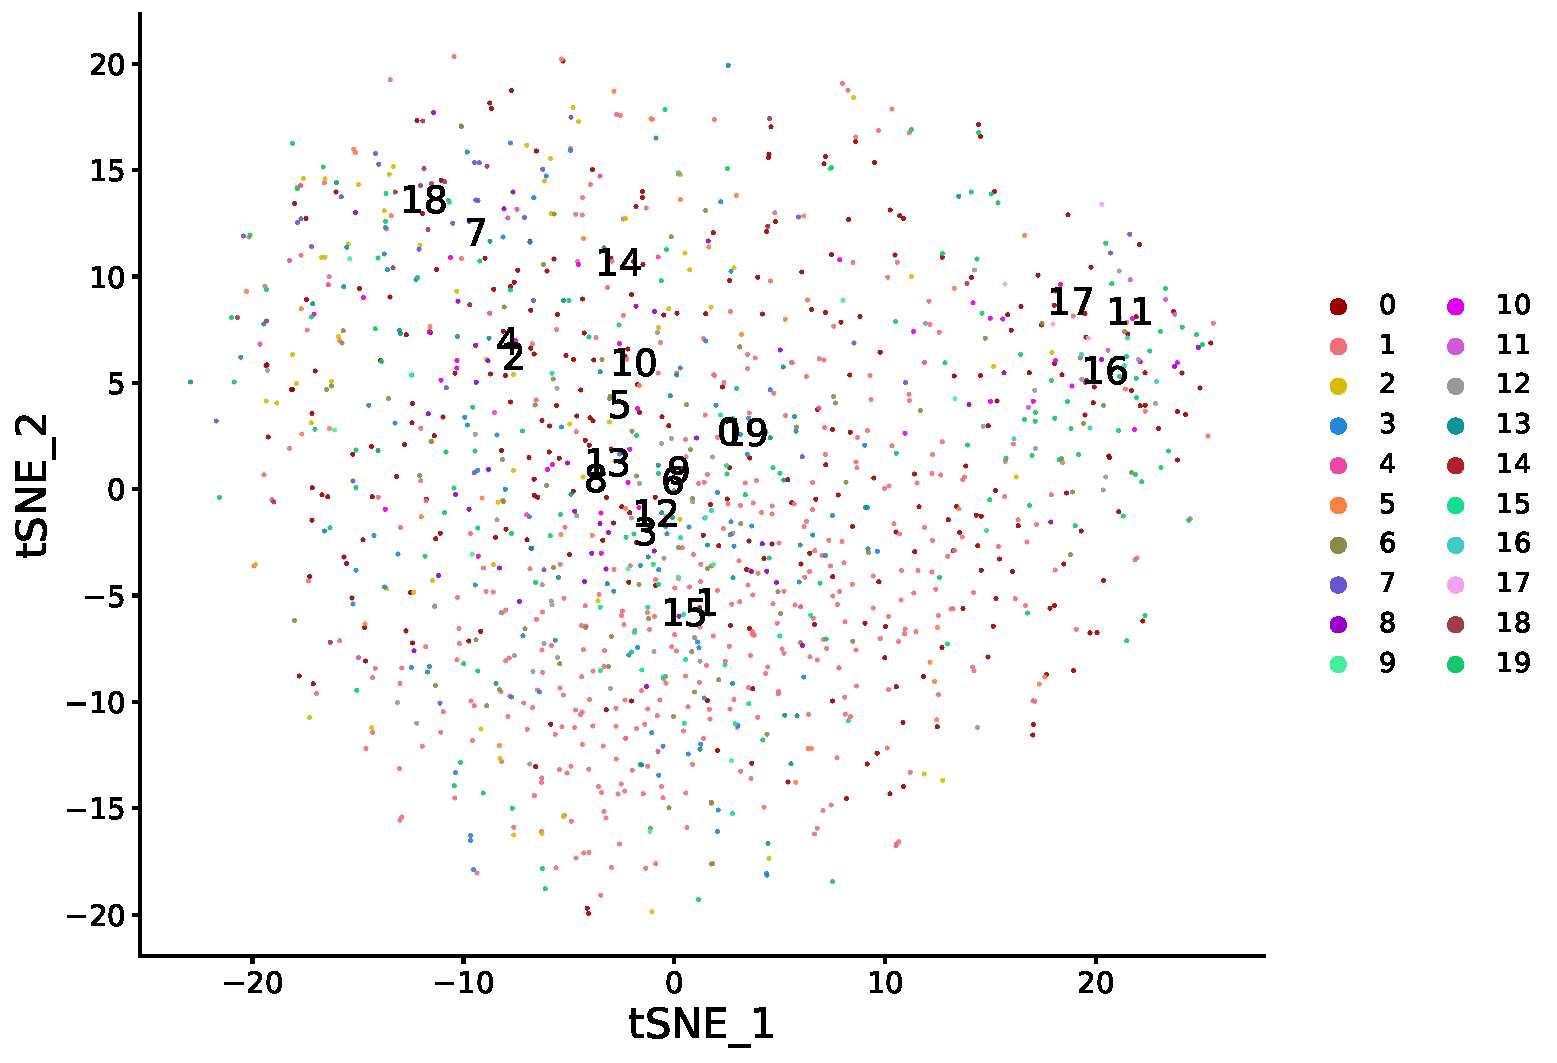
\includegraphics[width=0.40\linewidth]{fig_tsne_fedgmkd.pdf} \\[-2pt]
{\small (a) FedProto} & {\small (b) FedGMKD} \\[6pt]
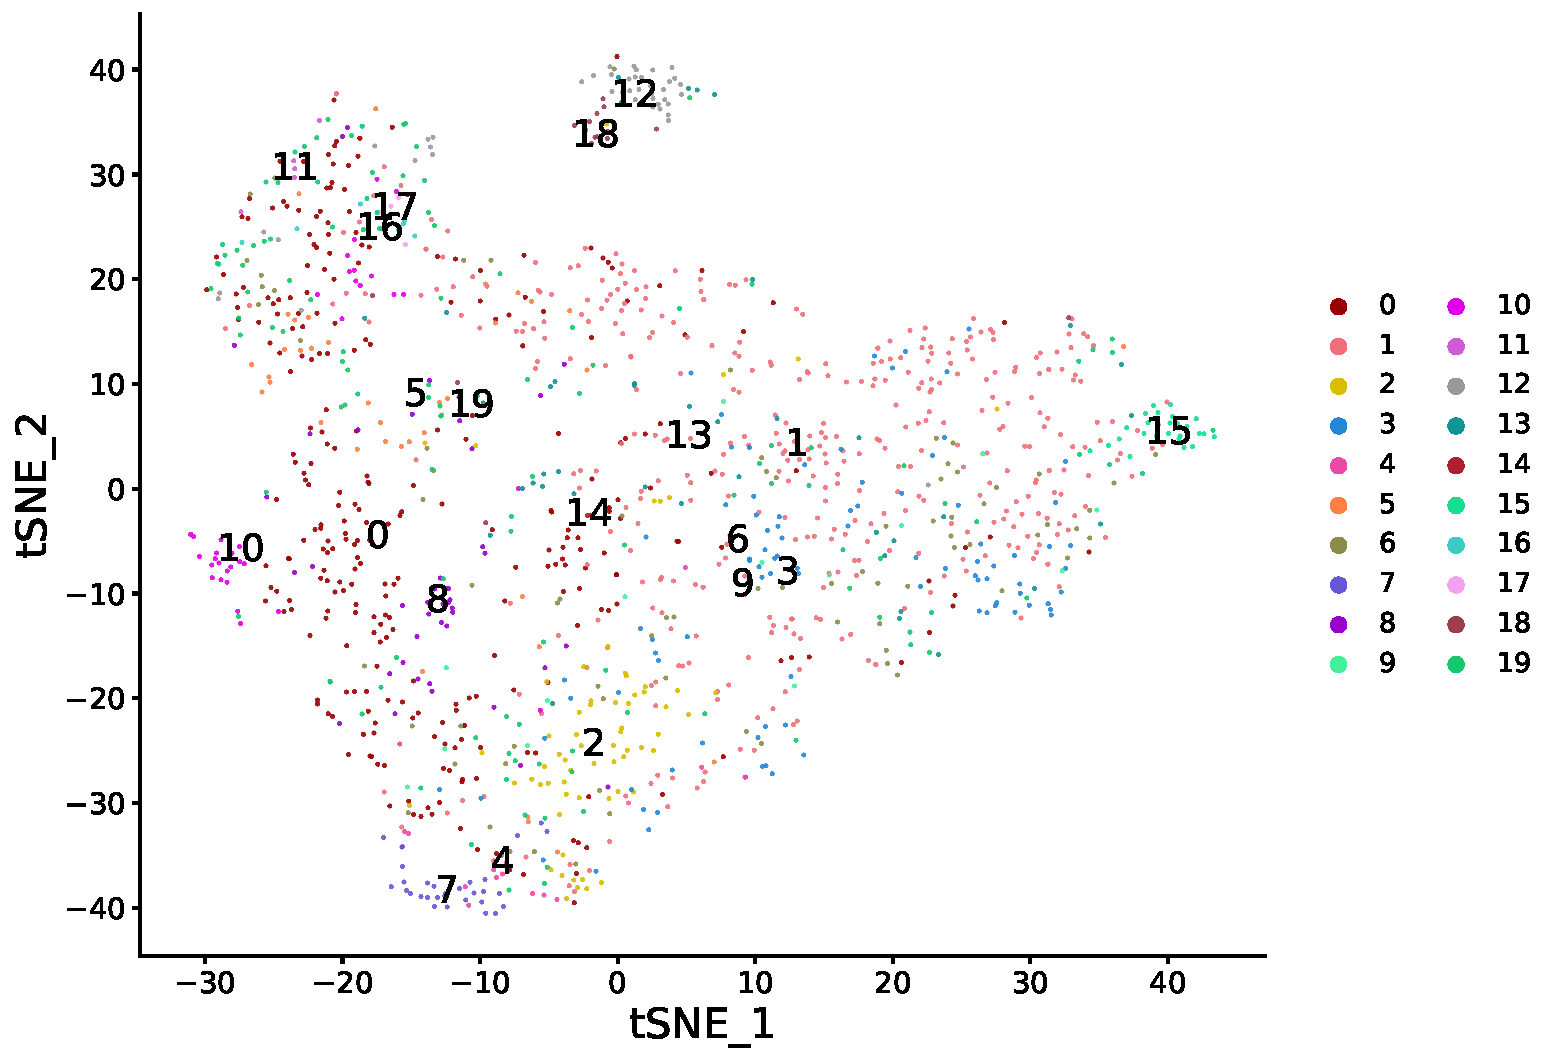
\includegraphics[width=0.40\linewidth]{fig_tsne_fedseproto.pdf} &
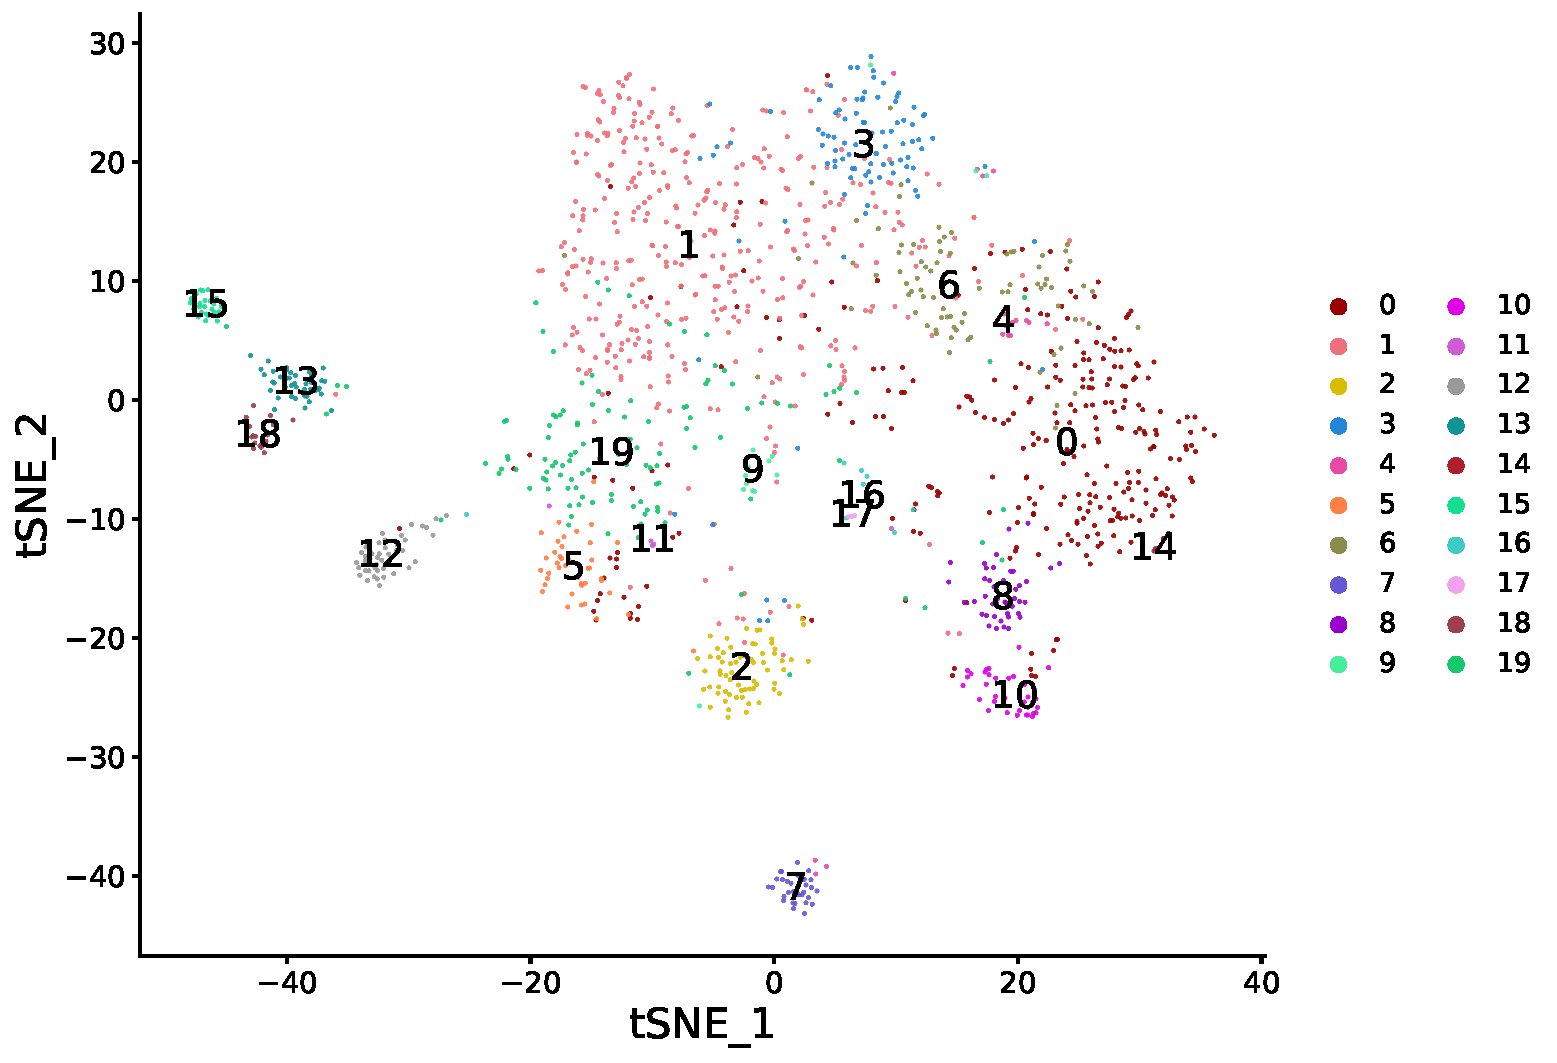
\includegraphics[width=0.40\linewidth]{fig_tsne_fedcop.pdf} \\[-2pt]
{\small (c) FedSeProto} & {\small (d) FedCoP (ours)}
\end{tabular}
\caption{t-SNE visualization of sample embeddings on MuReD (20 retinal pathology classes; marker color denotes class). FedCoP exhibits a structured layout where known co-occurring pathologies (e.g., diabetic retinopathy and macular edema) occupy adjacent regions---the geometric signature of $L_{co}$.}
\label{fig:tsne}
\end{figure*}

Figure~\ref{fig:tsne} reveals a qualitative difference in how the four prototype-based methods organize the embedding space. In all three baselines, class clusters are scattered with no apparent structure governing their relative positions: classes that clinically co-occur are not systematically near each other. FedCoP exhibits a visibly more structured layout where known co-occurring pathologies occupy adjacent embedding regions. This is the direct geometric effect of $L_{co}$: by aligning the prototype cosine Gram matrix to the federated co-occurrence correlation $\Rhat$, the loss actively pulls co-occurring diseases toward nearby directions and pushes mutually exclusive ones apart. Notably, this structure emerges despite no single client ever seeing all 20 classes ($\text{ways}{=}15$), providing empirical corroboration of Prop.~\ref{prop:estimation}(c).

\subsection{Ablation Study}
\label{sec:ablation}

We conduct a comprehensive ablation study toggling each component independently: federated vs.\ local vs.\ no co-occurrence structure, training-side $L_{co}$, inference-side mean-field decoder, distributional vs.\ point prototypes, entropy regularization, logit fusion ratio, distance metric, and temperature scaling. All variants share identical backbone, data split, and random seed. Table~\ref{tab:ablation} presents key ablations on ChestX-ray14; the full 36-configuration variant matrix is provided in the supplementary material.

\begin{table}[t]
\centering
\caption{Ablation results on ChestX-ray14. ``--'' denotes component removed from full FedCoP. The last row removes both sides of $\Rhat$ usage, equivalent to a distributional-prototype baseline without co-occurrence.}
\label{tab:ablation}
\footnotesize
\setlength{\tabcolsep}{3pt}
\begin{tabular}{lcccc}
\toprule
Variant & m-AUC & m-F1 & Ham. & Acc \\
\midrule
FedCoP (full)                  & \textbf{0.7053} & 0.2949 & \textbf{0.1956} & 0.9083 \\
~~--no co-occurrence ($\Rhat{=}I$) & 0.6938 & 0.2861 & 0.2112 & 0.8955 \\
~~--no $L_{co}$                 & 0.6981 & 0.2894 & 0.2038 & 0.9017 \\
~~--no MF decoder              & 0.7004 & 0.2911 & 0.2005 & 0.9048 \\
~~local $\Rhat$ (per-client)   & 0.6892 & 0.2803 & 0.2187 & 0.8901 \\
~~point prototypes             & 0.6965 & 0.2847 & 0.2089 & 0.8976 \\
~~no $L_{ent}$                 & 0.6944 & 0.2877 & 0.2091 & 0.8950 \\
\midrule
no $L_{co}$ + no MF decoder    & 0.6841 & 0.2724 & 0.2245 & 0.8843 \\
\bottomrule
\end{tabular}
\end{table}

\noindent\textbf{Federated $\Rhat$ vs.\ local vs.\ none.} Removing the co-occurrence structure entirely ($\Rhat{=}I$) drops macro-AUROC by 1.6\%. Notably, using \emph{per-client local} $\Rhat$ is \emph{worse} than using none at all (0.6892 vs.\ 0.6938), confirming Prop.~\ref{prop:estimation}(c): local co-occurrence estimates are biased and noisy under non-IID class partitioning, and injecting them at training time is actively harmful.

\noindent\textbf{Training-side $L_{co}$ vs.\ inference-side decoder.} Removing $L_{co}$ costs 1.0\% macro-AUROC; removing the decoder costs 0.7\%. Removing both simultaneously (last row) costs 3.0\%, confirming they are complementary mechanisms acting on different objects (prototype geometry vs.\ label probabilities) and are not redundant.

\noindent\textbf{Distributional vs.\ point prototypes.} Switching from diagonal Gaussian to point prototypes drops 1.2\%, confirming that per-client variance information matters for Bayesian fusion quality.

\noindent\textbf{Entropy regularizer.} Removing $L_{ent}$ drops 1.5\%, consistent with the hypothesis that variance collapse silently degrades distributional prototypes. The $L_{ent}$ guardrail is small but structurally important.

\noindent\textbf{Additional ablations.} The supplementary material includes full analyses of logit fusion ratio $\alpha$ (optimum at 0.5), temperature $T$ (best at 1.0), distance metric (Mahalanobis significantly outperforms Euclidean and cosine), EMA momentum ($\beta_{\text{ema}}{=}0.9$ optimal), structure warmup $W_{co}$ (below 5 rounds, early noisy $\Rhat$ degrades performance), and shrinkage $\eta$ (robust in $[0.05, 0.2]$, degraded outside).

% =====================================================================
\section{Conclusion}

We argued that pathology co-occurrence is an intrinsically federated quantity---invisible to any single client that sees only a subset of the $C$ classes and recoverable only by federated aggregation of label sufficient statistics---and we made it a first-class citizen of the federation. FedCoP estimates this structure through a privacy-safe, count-weighted, de-biased estimator and uses it on both sides of the pipeline: a structure loss $L_{co}$ that aligns prototype inter-class geometry to the estimated correlation, and a mean-field decoder that propagates diagnostic evidence across co-occurring classes at inference time.

The theoretical analysis establishes that the independent per-class sigmoid decoder---ubiquitous in prototype-based FL---is Bayes-optimal only under conditional independence and pays a second-order regret otherwise, and that the mean-field decoder is never worse and strictly improves as the coupling estimate approaches the true residual correlation. The federated estimator is provably unbiased under participation reweighting, concentrates at a parametric rate, and is formally unrecoverable by any single client under non-IID class partitioning.

Experiments on two multi-label medical datasets of different modalities confirm consistent improvements over five baselines, and comprehensive ablations (36 configurations) isolate the contribution of each component, confirming that the federated structure, the training-side geometry, and the inference-side evidence propagation each contribute independently and complementarily.

Two limitations warrant explicit mention. First, $\Rhat$ approximates rather than equals the residual label correlation $\Sigmay$; the shrinkage term hedges this mismatch conservatively, but a feature-conditional estimator would tighten the theory--practice gap. Second, the single-client non-recoverability argument assumes strict subset class supports; when hospital class supports overlap substantially, local co-occurrence estimates become partially informative and the federated gain narrows proportionally---a continuum the current theory bounding only the extremes. Extending the estimator to the feature-conditional regime and to dynamic, streaming client participation are natural directions for future work.

% =====================================================================
% REFERENCES
\bibliographystyle{IEEEtran}
\bibliography{FedCoP_wacv}

\end{document}
